% TODO textcommand für Scenegraph-Ebene, SimpleMesh-Ebene, Icon-Ebene

\newpage
\section{Umsetzung des Prototyps}\label{sec:RealizationOfPrototype}
Im Folgenden wird das \gls{Mockup}, die Implementierung und das Deployment des Prototyps beschrieben. Während der Skizzierung der \gls{Mockup}s und der Implementierung wurde auf eine gute Benutzerfreundlichkeit geachtet. Hierfür wurde sich unter anderem an Nielsens Usability Heuristics \cite{Nielsen.1994} orientiert. Im Abschnitt \ref{sec:UsabilityHeuristics} wird genauer geprüft wie gut diese eingehalten wurden.

\subsection{Mockup}\label{sec:Mockup}
Für den Prototyp wurden \gls{Mockup}s skizziert die während der Implementierung als Orientierungshilfe genutzt wurden. Diese \gls{Mockup}s wurden zunächst auf Papier niedergeschrieben und für die folgende Beschreibung mithilfe von Figma \cite{Figma} digitalisiert. Es gibt jeweils ein \gls{Mockup} für die Übersicht, Steuerung und Verwaltung, sowie für das Routenplanungs-Popup in der Steuerung. Für den Editiermodus wurde kein \gls{Mockup} entworfen, da das Design und Verhalten zu stark von den Möglichkeiten in \deckgl{} abhängt, die noch nicht vollständig bekannt waren, als die \gls{Mockup}s entworfen wurden. Stattdessen wurde das Design und Verhalten des Editiermodus während der Implementierung festgelegt.

Die Abbildung \ref{fig:MockupOverview} im Anhang zeigt das \gls{Mockup} für die Übersicht. In der Übersicht werden die Raummodelle zusammen mit den verschiedenen Roboterdaten angezeigt. So werden die Standorte mithilfe von Icons, die Roboterpfade mithilfe von Linien und die Roboterpositionen mithilfe von 3D-Modellen der Roboter dargestellt. Es gibt außerdem Buttons mit denen zwischen den verschiedenen Stockwerken navigiert werden kann und mit denen die Roboter ausgewählt werden können. Zusätzlich gibt es einen Button, der es ermöglicht den ausgewählten Roboter automatisch zu verfolgen und einen anderen Button, mit dem die Kameraposition wieder zur Ausgangsposition zurückgesetzt werden kann. Die Buttons sind abhängig von ihren Funktionen in den vier Ecken der Anwendung gruppiert.

Die Steuerung erweitert die Übersicht nur um weitere Funktionen und unterscheidet sich daher kaum von dieser. Abbildung \ref{fig:MockupControls} im Anhang zeigt das \gls{Mockup} der Steuerung. Der einzige Unterschied zur Übersicht sind die zusätzlichen Buttons mit denen eine Lieferroute bestimmt, der Roboter zum Aufladen geschickt und der aktuelle Lieferauftrag abgebrochen werden kann. Die Abbildung \ref{fig:MockupRoutePlanner} im Anhang zeigt das \gls{Mockup} für das Routenplanungs-Popup das sich öffnet, wenn der Lieferroute-Button ausgewählt wird. In dem Popup muss ein Ziel und ein Roboter ausgewählt werden, bevor der Auftrag gestartet werden kann. Um die Routenerstellung zu vereinfachen, sollen sowohl Roboter als auch Standorte zusätzlich über das Anklicken auf der Karte auswählbar sein.

Die Abbildung \ref{fig:MockupAdministration} zeigt das \gls{Mockup} für die Verwaltung. Hier gibt es jeweils eine Liste für die Roboter und die Stockwerke. In der Liste der Roboter können verschiedene Informationen der einzelnen Roboter, wie beispielsweise der systeminterne \ac{ID} und die tägliche Neustartzeit ausgelesen werden. Auch können Einstellungen der Roboter, wie Name und Ausgabepunkt geändert werden. Zudem gibt es für jeden Roboter eine Vorschau der Übersicht, in der die Position des Roboters gezeigt wird. Sowohl in der Liste der Roboter als auch in der Liste der Stockwerke gibt es für jedes Stockwerk eine Auflistung der Standorte. In der Liste der Stockwerke gibt es außerdem eine Vorschau der Übersicht und zusätzlich ein Kontextmenü, über das in den Editiermodus des Stockwerks gewechselt werden kann.

\subsection{Implementierung}
Es wurde ein Frontend entwickelt, dass auf das \ac{BCB} zugreift, um die Roboterdaten anzufragen. Wie das \ac{BCB} hierbei mit den Robotern kommuniziert, wird im Abschnitt \ref{sec:BotControlBackend} erklärt. Das Frontend nutzt das Web-Framework React mit \ac{HTML}, \ac{Sass} und TypeScript. Die Vorteile von TypeScript und \ac{Sass} gegenüber JavaScript und \ac{CSS}, wie auch das Web-Framework React werden im Abschnitt \ref{sec:WebTechnologies} genauer erläutert. Zustandsinformationen die React-Komponenten übergreifend abgerufen werden, werden zentral mithilfe von Redux gespeichert. Die Grundstruktur des Frontend-Projekts wurde mithilfe des Shell Befehls npx create-chayns-app \cite{CreateChaynsApp} aufgesetzt. Die Kompilierung ist mithilfe des \ac{npm}-Pakets chayns-toolkit \cite{ChaynsToolkit} konfiguriert. \ac{GUI}-Elemente wie Buttons und Aufklapper werden durch die Komponentenbibliothek chayns-components \cite{ChaynsComponents} bereitgestellt. Außerdem werden die \ac{npm}-Pakete clsx \cite{clsx} und fortawesome \cite{fontawesome} genutzt. Mithilfe von clsx lassen sich \ac{HTML}-Klassennamen dynamisch anwenden. Das fortawesome \ac{npm}-Paket wird genutzt, um \ac{SVG} Icons als Zeichenkette zu importieren.

\subsubsection{Übersicht}
In der Übersicht werden die Roboterdaten in Kombination mit den Gebäudemodellen mithilfe von \deckgl{} angezeigt. Hierfür werden verschiedene Ebenen eingesetzt. Auch bietet die Übersicht eine Echtzeitaktualisierung der Roboter und Interaktivität für den Nutzer.

\paragraph{Gebäudemodelle}
Für den Prototyp sind die \ac{URL}-Verweise der 3D-Modelle hartkodiert, oder in anderen Worten in den Quelltext der Webanwendung eingebettet. Für ein potenzielles Produktivsystem müssten die \ac{URL}-Verweise in der Datenbank des \ac{BCB}s abgespeichert werden. Die Modelle sind im chanys.space gespeichert, nutzen – aus Gründen, die im Abschnitt \ref{sec:ModelFileFormat} erläutert werden – das \ac{glTF}-Format und werden über die ScenegraphLayer angezeigt. Diese Ebene ist dafür ausgelegt, ein bestimmtes 3D-Modell beliebig oft an verschiedenen Positionen anzuzeigen \cite{DeckglScenegraphLayer}, was auf die Hauptfunktion von \deckgl{} – die Visualisierung riesiger Geodaten Mengen \cite[S.~3]{YangWang2019} – zurückzuführen ist. Unterschiedliche 3D-Modelle lassen sich nicht in einer ScenegraphLayer-Instanz einbinden, weshalb für jedes 3D-Modell eine eigene Instanz der ScenegraphLayer erzeugt werden muss. \deckgl{} ist für den Einsatz von über 100 Ebenen gleichzeitig ausgelegt, wobei wahrscheinlich sogar der Einsatz von bis zu 1000 Ebenen ohne große Performance Einbußen möglich ist \cite{DeckglPerformance}. Im Prototyp besteht ein Stockwerk aus bis zu sechs 3D-Modellen und somit auch aus bis zu sechs ScenegraphLayers, wehalb davon auszugehen ist, dass nie mehr als 100 Modelle für die Darstellung eines Stockwerks erforderlich sind. In Anbetracht dessen, dass nie mehrere Stockwerke gleichzeitig angezeigt werden, ist es unwahrscheinlich, dass die beschriebene mehrfache Verwendung der Ebene negative Auswirkungen auf die Performance hat. Für die Ebenen ist das Backface Culling aktiviert. Mithilfe vom Backface Culling werden die von der Kamera weg gerichteten Polygone ausgeblendet \cite{BackfaceCulling}. Meist wird Backface Culling genutzt, um Polygone auszublenden, die sowieso hinter anderen Polygonen versteckt sind, wodurch die Darstellungsgeschwindigkeit erhöht wird. Im Fall der Gebäudemodelle sind die Polygone in den Raum hineingerichtet. Somit bewirkt das Backface Culling, dass die Wände und Decken, die dem Nutzer die Sicht in den Raum verdecken, ausgeblendet werden. In der Abbildung \ref{fig:BackfaceCulling} wird dieser Effekt deutlich. So sieht man auf der linken Seite, dass ohne das Backface Culling nicht von außen in den Raum hineingesehen werden kann, während es auf der rechten Seite mit aktiviertem Backface Culling möglich ist.

\begin{figure}[H]
    \caption{Raummodell ohne und mit Backface Culling}\label{fig:BackfaceCulling}
    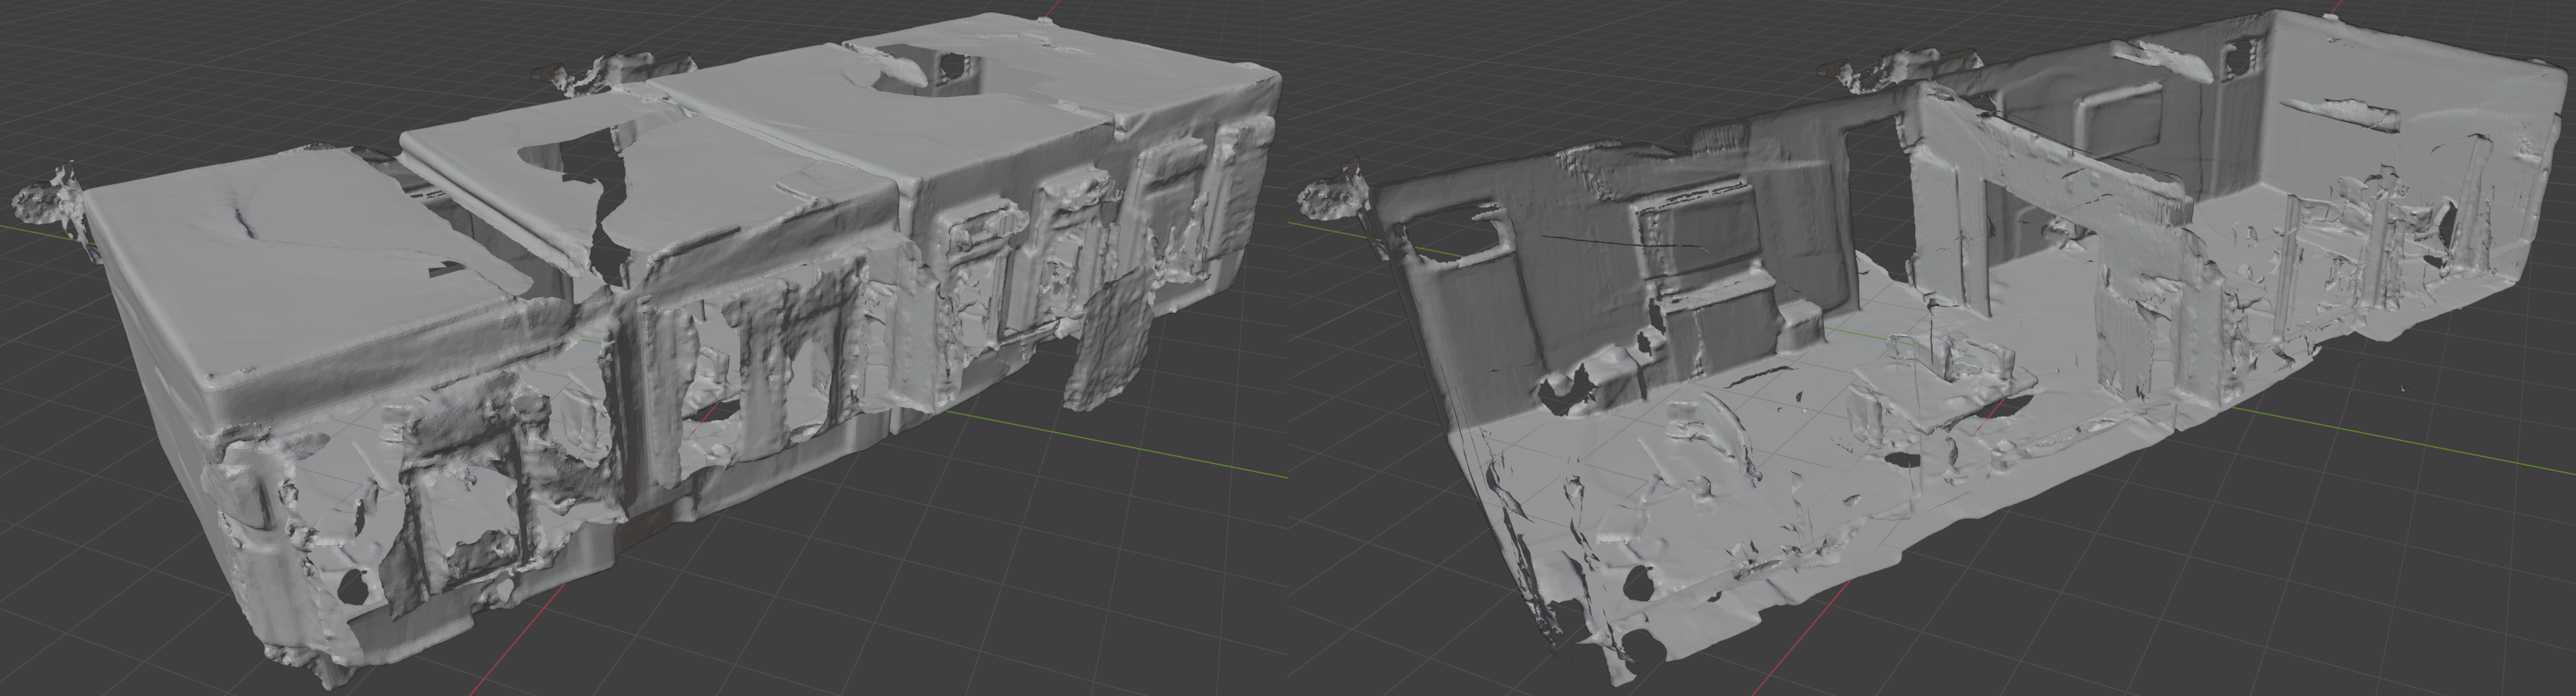
\includegraphics[width=0.9\textwidth]{Backface Culling Vergleich.png}
    \\
    Quelle: Eigene Darstellung
\end{figure}

\paragraph{Roboterdaten}\label{sec:RobotData}
Die Roboterdaten werden über verschiedene Endpunkte des \ac{BCB}s abgerufen. So gibt es einen Endpunkt für die Bezeichnungen der verschiedenen Standorte und einen Endpunkt für den Roboterstatus, Lieferauftrag und die Roboterposition \cite{BCBSwagger}. Für die Positionen aller Standorte und Roboterpfade gibt es keinen Endpunkt. Stattdessen können die Standorte und Pfade nur von Stockwerken angefragt werden, in denen sich zu dem Zeitpunkt Roboter befinden. Damit immer alle Daten aus allen Stockwerken abgerufen werden können, sind diese Daten im Prototyp für alle Stockwerke hartkodiert. Für ein potenzielles Produktivsystem müssten diese Daten in der Datenbank des \ac{BCB}s gespeichert und regelmäßig mit den Robotern synchronisiert werden.
% TODO Braucht es ein Schaubild, in dem die erweiterte Datenbankstrukur dargestellt wird?

Im Gegensatz zu den Gebäuademodellen werden die Robotermodelle im \ac{OBJ}-Format mit der SimpleMeshLayer \cite{DeckglSimpleMeshLayer} angezeigt. Mit der ScenegraphLayer gibt es das Problem, dass die Positionsänderungen der Modelle nicht animiert werden können, wodurch die SimpleMeshLayer brauchbarer, aber auch nicht ideal, ist. Laut der Dokumentation von \deckgl{} sollte das Animieren über die transition Property in allen Ebenen möglich sein \cite{DeckglLayerClass}. Deshalb handelt es sich bei dem Problem mit der ScenegraphLayer vermutlich um einen Bug. Wie im Abschnitt \ref{sec:ModelFileFormat} erwähnt, lässt sich die Materialdatei des \ac{OBJ} Formats nicht in der SimpleMeshLayer einbinden, weshalb die Roboter einfarbig angezeigt werden müssen. Das ist nicht unbedingt ein Nachteil, denn so können die Roboter durch eine herausstechende Farbe für den Nutzer besser sichtbar gemacht werden. Die Positionsänderungen der Roboter werden über die transitions Property animiert \cite{DeckglLayerClass}. Allerdings lässt sich die Rotationsänderungen nicht animieren, was vermutlich auch auf einin \deckgl{} zurückzuführen ist.

Über den Robotermodellen wird mithilfe der IconLayer der aktuelle Status der Roboter angezeigt. Während in einer ScenegraphLayer-Instanz nur ein bestimmtes 3D-Modell angezeigt werden kann, können in einer IconLayer-Instanz mithilfe der getIcon Zugriffsfunktion verschiedene Bilder angezeigt werden \cite{DeckglIconLayer}. So reicht im Gegensatz zur ScenegraphLayer eine IconLayer-Instanz aus, um alle Icons anzuzeigen. Die genutzten Icons stammen aus der Icon-Bibliothek Fontawesome und werden aus dem fortawesome \ac{npm}-Paket als \ac{SVG}-Zeichenkette importiert. Da die IconLayer \ac{SVG}-Zeichenketten nicht unterstützt, werden diese in das Data-\ac{URL} Format umgewandelt. Das Data-\ac{URL} Format kann Daten als \gls{Base64}-Zeichenkette innerhalb einer \ac{URL} einbetten \cite{DataUrlSpec}, was von der SimpleMeshLayer ausgelesen werden kann \cite{DeckglIconLayer}.

Die verschiedenen Standorte werden über eine weitere IconLayer-Instanz angezeigt. Wie bei den Roboter-Zuständen werden hierfür verschiedene Fontawesome-Icons genutzt. Wurde ein Roboter ausgewählt und hat dieser einen Lieferauftrag, dann wird der Zielstandort farbig markiert. Die Pfade und virtuellen Wände werden über eine Instanz der PathLayer \cite{DeckglPathLayer} dargestellt. Die virtuellen Wände werden gestrichelt und in einer anderen Farbe angezeigt, damit diese von den Roboterpfaden unterschieden werden können. Für die gestrichelte Darstellung wird die PathStyleExtension \cite{DeckglPathStyleExtension} genutzt. Der Boden der 3D-Modelle liegt relativ konstant auf der z-Koordinate – der vertikalen Position – 0. Aufgrund der Ungenauigkeiten die durch den \ac{LiDAR}-Scan entstehen ist der Boden der 3D-Modelle nicht vollständig eben. Da die Positionen der Roboterdaten zweidimensional sind, und somit keine vertikale Position haben, besteht die Gefahr, dass diese an manchen Stellen unter dem Boden der 3D-Modelle verschwinden, wenn sie auf der z-Koordinate 0 angezeigt werden. Aus diesem Grund werden die Icons und Pfade an einer leicht erhöhten z-Koordinate positioniert.

Bei der Abbildung \ref{fig:OverviewScreenshot} handelt es sich um einen Screenshot aus der Übersicht im Prototyp. Man sieht alle erwähnten Ebenen, sowie die verschiedenen Buttons. Basierend auf dem Feedback aus den Usability Tests, die im Abschnitt \ref{sec:UsabilityTests} genauer beschrieben werden, wurden Buttons ergänzt, die es nicht im \gls{Mockup} gibt.

\begin{figure}[H]
    \caption{Übersicht}\label{fig:OverviewScreenshot}
    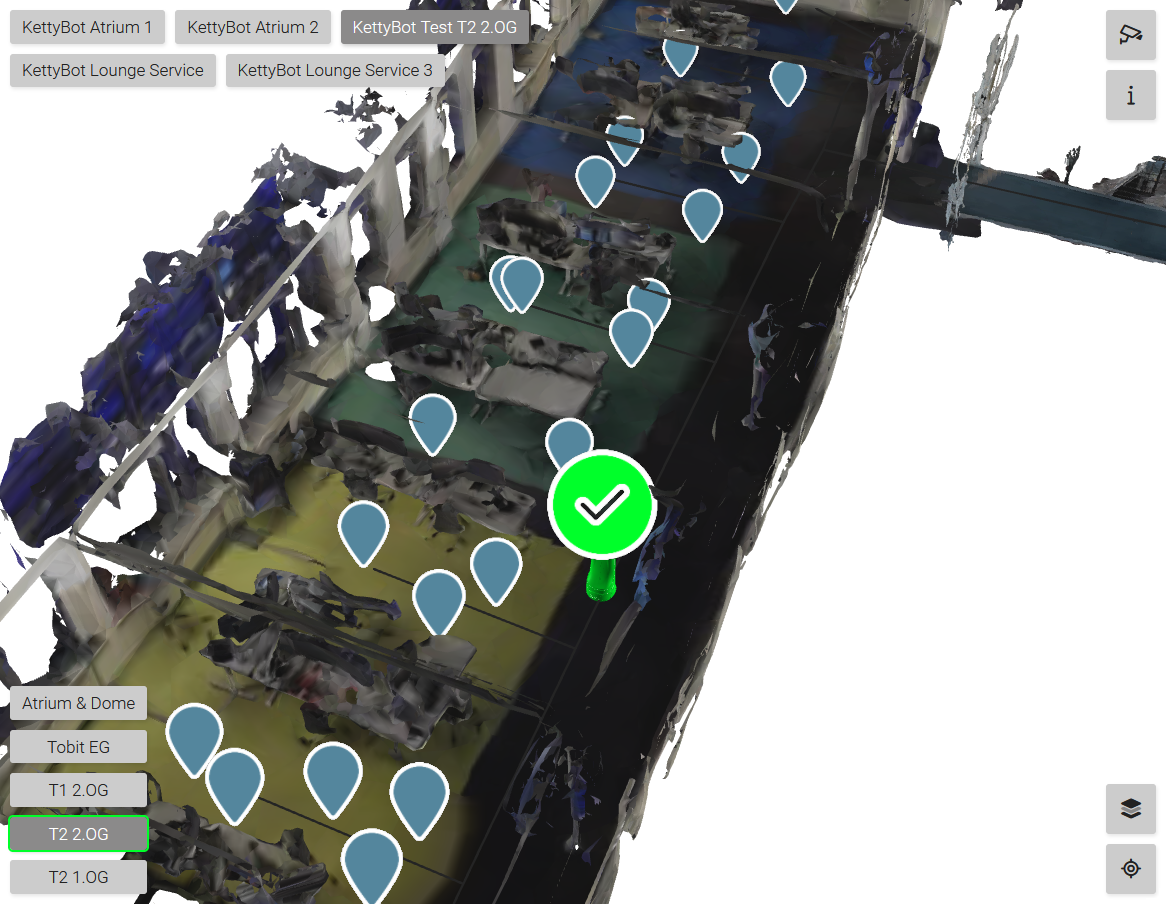
\includegraphics[width=0.9\textwidth]{Screenshot Uebersicht.png}
    \\
    Quelle: Eigene Darstellung
\end{figure}

\paragraph{Echtzeit-Aktualisierung}
Die Positionen sowie weitere Statusinformationen der Roboter, wie beispielsweise der aktuelle Auftrag und Akkuladung, werden mithilfe einer indirekten Verbindung zwischen der Webanwendung und dem \ac{BCB} regelmäßig aktualisiert. Hierfür wird der im Abschnitt \ref{sec:Chayns} erwähnte \gls{Websocket}-Service genutzt. In der Abbildung \ref{fig:RobotStatusUpdate} ist der Ablauf einer Statusaktualisierung vereinfacht dargestellt. Aktualisiert ein Roboter seine Position, wird die entsprechende Information an das \ac{BCB} gesendet. Wie die Kommunikation zwischen Robotern und \ac{BCB} funktioniert wird im Abschnitt \ref{sec:BotControlBackend} erklärt.
% Passt das so? Funktioniert MQTT wie beschrieben?
Das \ac{BCB} sendet daraufhin eine Nachricht an den \gls{Websocket}-Service, der diese Information wiederum an alle verbundenen Clients schickt, die Nachrichten des \ac{BCB}s erwarten. So sieht man in der Abbildung auch, dass der dritte Client keine Nachricht empfängt, da er Nachrichten eines anderen Systems erwartet.

\begin{figure}[H]
    \centering
    \caption{Kommunikationsweg von Statusaktualisierungen der Roboter}\label{fig:RobotStatusUpdate}
    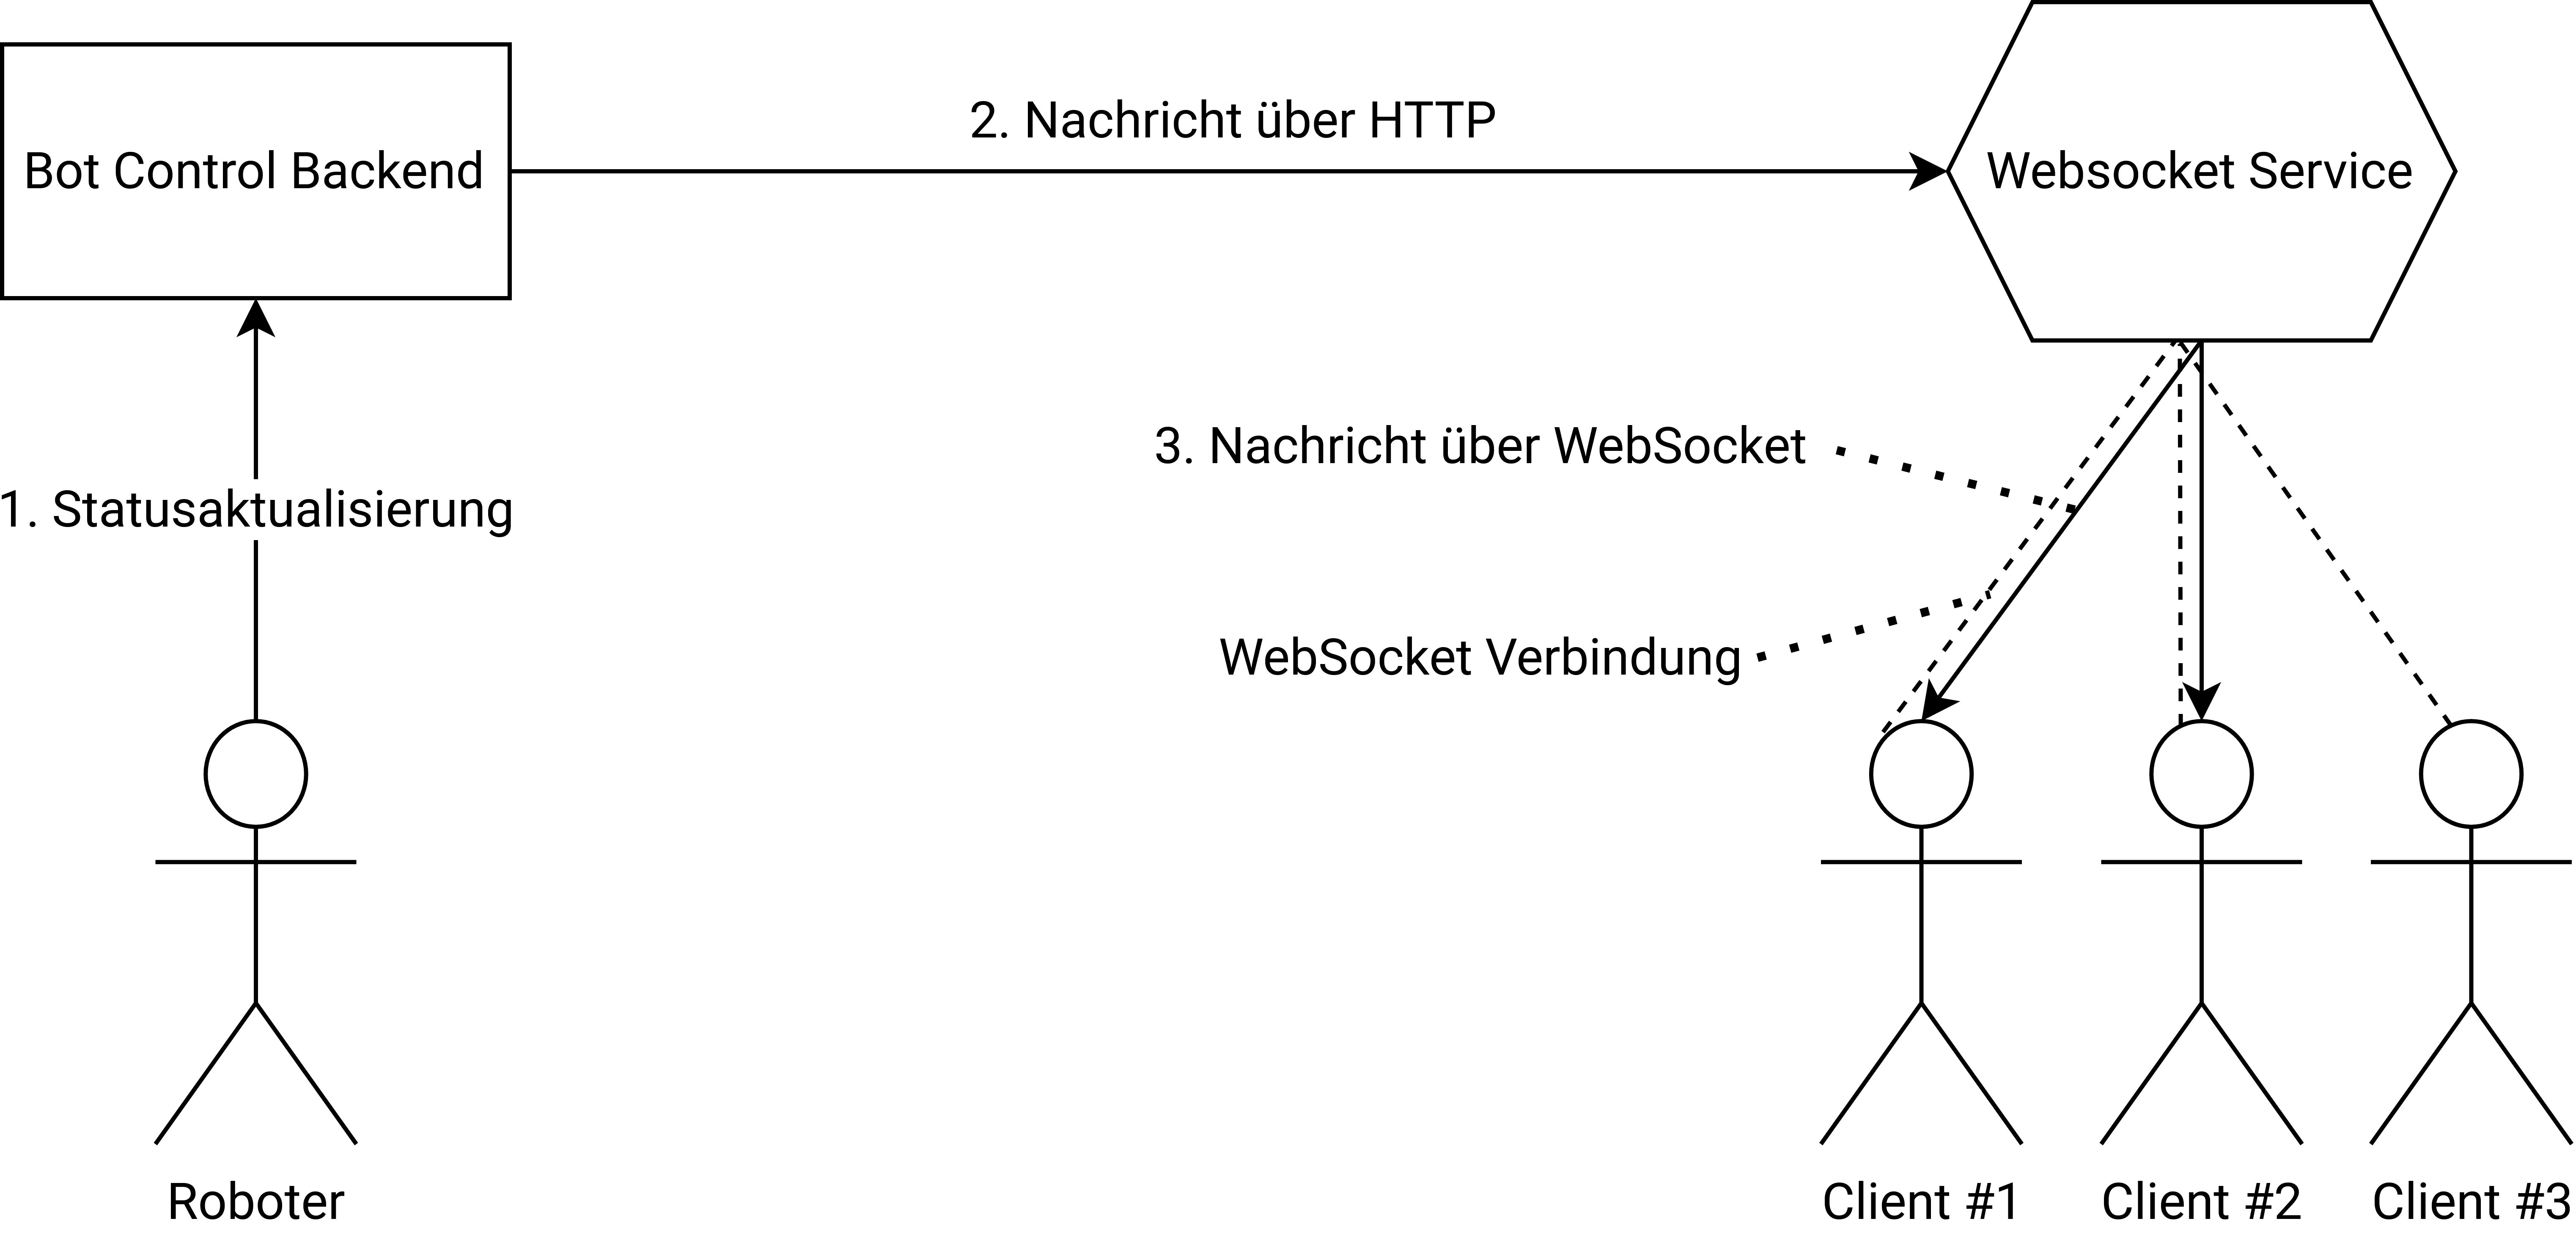
\includegraphics[width=0.9\textwidth]{Websocket Service.png}
    \\
    Quelle: Eigene Darstellung
\end{figure}

Die über den \gls{Websocket}-Service empfangene Statusaktualisierung wird zentral im Redux-Store gespeichert, sodass dem Nutzer direkt die aktualisierten Informationen angezeigt werden können.

\paragraph{Interaktion}
Die Roboter, sowie die Standorte sind mithilfe der onClick Property der entsprechenden Ebene \cite{DeckglInteractivity} auswählbar. Ausgewählte Standorte und Roboter werden verfärbt angezeigt. Außerdem erscheint beim Auswählen eines Roboters ein Button über den sich weitere Informationen wie die Akkuladung anzeigen lassen. Schwebt die Maus über einem Standort oder Roboter, dann wird mithilfe der getTooltip Property \cite{DeckglDeckClass} ein Tooltip angezeigt, in dem der Name des entsprechenden Objekts und weitere wichtige Informationen stehen. Es gibt zudem einen Button, über den einem Roboter gefolgt werden kann. Die Kamera wird hierfür durch den FlyToInterpolator \cite{DeckglFlyToInterpolator} zum ausgewählten Roboter bewegt. Beim Folgen eines Roboters wird die Kameraposition mithilfe der transitionDuration Property \cite{DeckglAnimationsAndTransitions} animiert.

\subsubsection{Steuerung}
Wie im Abschnitt \ref{sec:Mockup} beschrieben, gibt es drei Aktionen die zum Steuern der Roboter ausgeführt werden können: Lieferauftrag, Laden und Abbrechen. Mit dem Laden und Abbrechen wird der aktuelle Lieferauftrag abgebrochen, worauf der Nutzer auch über einen Bestätigungsdialog hingewiesen wird. Für das Starten eines Lieferauftrags muss ein Ziel und ein Roboter angegeben werden. Hierfür gibt es Inputs, mit denen nach Standorten und Robotern gesucht werden kann. Bei den Inputs handelt es sich um die PersonFinder React-Komponente \cite{ChaynsPersonFinder} der chayns-components, die eigentlich für die Suche nach chayns Nutzern genutzt wird, im Prototyp aber für die Suche nach Robotern und Standorten konfiguriert ist. Das Ziel und der Roboter lassen sich außerdem über das Anklicken auf der Karte auswählen. Die Roboter können zudem über ihre Buttons ausgewählt werden. Bestimmte Standorte wie Türen oder Fahrstühle können nicht als Zielstandorte ausgewählt werden. Aus diesem Grund sind diese weder im Input und noch auf der Karte auswählbar. Zum endgültigen Ausführen der drei Aktionen werden die entsprechenden Endpunkte Robot/Call, Robot/Charge und Robot/Cancel im \ac{BCB} \cite{BCBSwagger} aufgerufen. Die Abbildung \ref{fig:ControlsScreenshot} zeigt die Steuerung und das Routenplanungs-Popup. Im Popup sind bereits Ziel und Roboter eingestellt. Der ausgewählte Standort ist auf der Karte farblich markiert.

\begin{figure}[H]
    \caption{Steuerung und Routenplanung}\label{fig:ControlsScreenshot}
    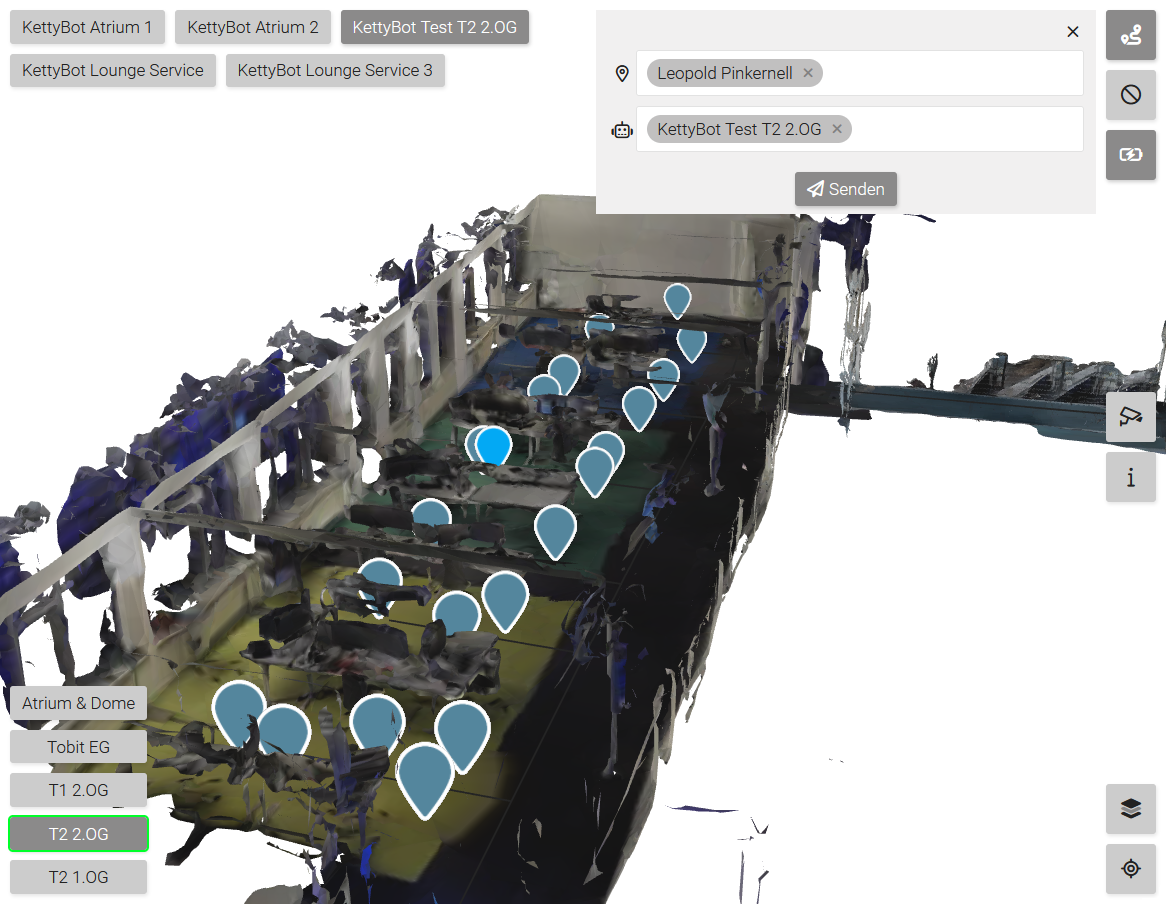
\includegraphics[width=0.9\textwidth]{Screenshot Steuerung.png}
    \\
    Quelle: Eigene Darstellung
\end{figure}

\subsubsection{Verwaltung}
Die Verwaltung ist nicht besonders komplex, da die Daten der Roboter und Stockwerke in jeweils einem Array strukturiert sind und somit leicht mithilfe von React gemappt werden können. Hiermit ist gemeint, dass die Arrays mithilfe der map Funktion zu Arrays an React-Komponenten umgewandelt werden können, die daraufhin gerendert werden können \cite[S.~35-36]{Boduch2020}.

In der Roboterliste werden im Gegensatz zum \gls{Mockup} mehr Statusinformationen angezeigt. Auch können mehr Einstellungen der Roboter geändert werden. Da die Übersicht der verschiedenen Standorte auch über die Liste der Stockwerke ersichtlich ist und dadurch redundant ist, wurde diese aus der Roboterliste entfernt. Bei der Abbildung \ref{fig:RobotlistScreenshot} handelt es sich um einen Screenshot der Verwaltung im Prototyp. Man sieht einen geöffneten Roboter-Eintrag, das Kontextmenü, über das Einstellungen geändert werden können und einen Tooltip, in dem eine Statusinformation erläutert wird.

\begin{figure}[H]
    \caption{Verwaltung}\label{fig:RobotlistScreenshot}
    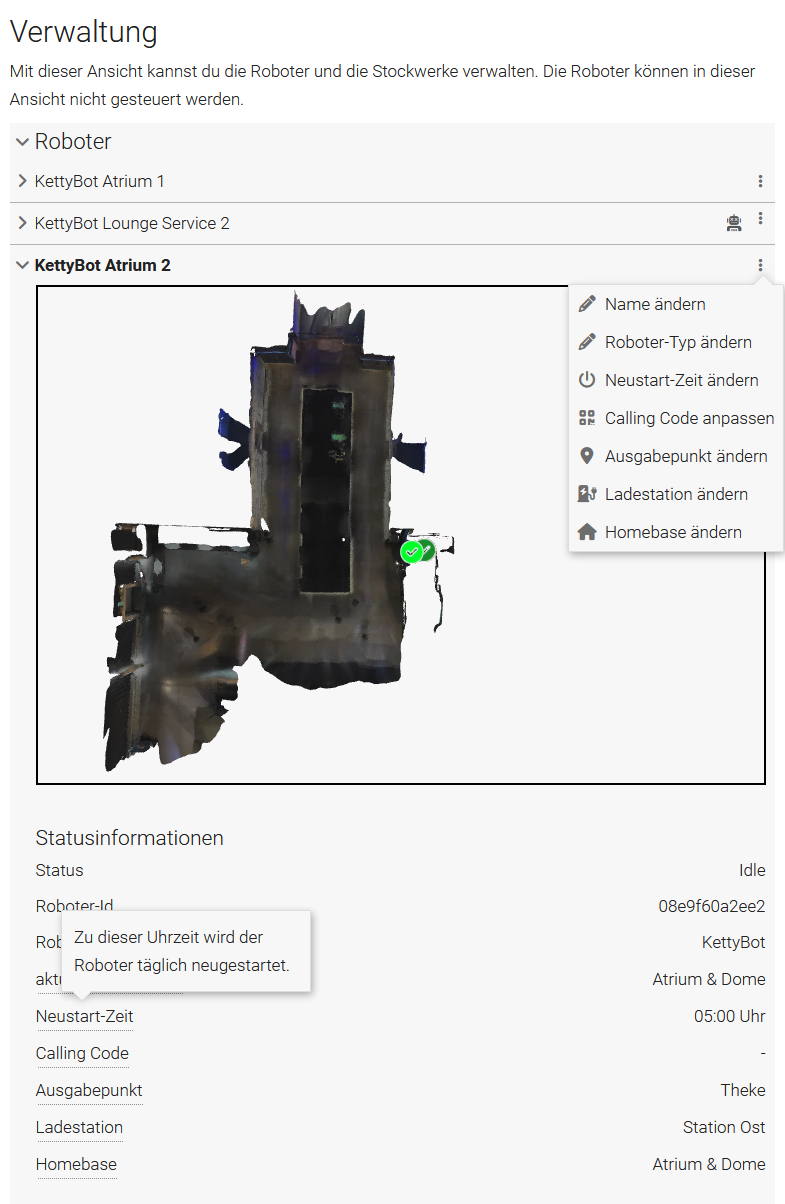
\includegraphics[width=0.6\textwidth]{Screenshot Verwaltung.png}
    \\
    Quelle: Eigene Darstellung
\end{figure}

Die Stockwerkliste unterscheidet sich nur geringfügig vom \gls{Mockup}. So werden die Standorte im Gegensatz zum \gls{Mockup} gruppiert nach der Art des Standorts aufgelistet. Diese Gruppierung ist hilfreich, da die Art des Standortes nicht unbedingt aus dem Namen ersichtlich ist.

Sowohl in der Roboter- als auch in der Stockwerkliste gibt es eine Vorschau des entsprechenden Stockwerks, um die Position des Roboters oder die Positionen der Standorte zu zeigen. Hierbei handelt es sich um die Nutzeransicht mit reduzierten Funktionen. Die Vorschau ist im \gls{Mockup} automatisch geöffnet, was ein Problem ist, da die entsprechende \deckgl{}-Karteninstanz – aufgrund des Verhaltens der genutzten Aufklapper-Komponente – beim Öffnen des Aufklappers initialisiert wird. Die Initialisierung der \deckgl{} Karteninstanz ist rechnerisch aufwändig und verursacht beim ersten Öffnen des Aufklappers starke Ruckler in der Aufklapper-Animation. Um diese Ruckler zu verhindern wird ein Button angezeigt, über den die Karte manuell initialisiert werden kann. Dadurch gibt es die Ruckler beim Klicken des Buttons und nicht beim Öffnen des Aufklappers, was weniger störend ist.

\subsubsection{Editiermodus}\label{sec:EditMode}
In der Verwaltung, sowie in der Nutzeransicht gibt es die Möglichkeit in den Editiermodus eines Stockwerks zu wechseln. In diesem können die Roboterdaten und 3D-Modelle manuell synchronisiert werden. Der Editiermodus ähnelt der Nutzeransicht und unterscheidet sich nur durch andere Buttons und die Editiermöglichkeiten. Da der Einsatz der Steuerungs- und Umschalttaste nötig ist, kann dieser Modus nicht an Mobilgeräten genutzt werden. Im Editiermodus hat der Nutzer die Möglichkeit neue 3D-Modelle zu importieren. Hierfür gibt es einen einfachen Dateiinput der nur Dateien im \glb{} Format akzeptiert. Wie bereits erwähnt sind die 3D-Modelle im Prototyp hartkodiert. Entsprechend werden Änderungen sowie neu importierte 3D-Modelle nur für die aktuelle Sitzung gespeichert und gehen verloren, wenn die Anwendung erneut geöffnet und somit eine neue Sitzung gestartet wird. Mithilfe der in \deckgl{} integrierten Events onDragStart, onDrag und onDragEnd \cite{DeckglInteractivity} kann das angeklickte 3D-Modell per Ziehen der Maus verschoben und rotiert werden. So wird das ausgewählte Modell beim Ziehen entweder verschoben oder rotiert, je nachdem ob die Steuerungs- oder Umschalttaste gedrückt wurde. Das Verschieben und Rotieren kann mithilfe der Tastenkombination Strg + Z rückgängig gemacht und mit Strg + Y wiederholt werden. Hierfür sind zwei Stapelspeicher implementiert in denen die vergangenen und rückgängig gemachten Aktionen per push hinzugefügt und per pop wieder herausgenommen werden. Bei Abbildung \ref{fig:EditmodeScreenshot} handelt es sich um einen Screenshot des Editiermodus. Oben Links sind die Buttons zum rückgängig machen und wiederhohlen. Mit dem Button oben rechts kann die initiale Kameraposition geändert werden. Unten rechts sind Buttons zum Importieren neuer Modelle – wobei das Importieren nicht implementiert ist –, zum Anzeigen verschiedener Tastenkombinationen und zum Zurücksetzen der Kameraposition. Außerdem gibt es unten Buttons zum Speichern und Abbrechen des Editierens.

\begin{figure}[H]
    \caption{Editiermodus}\label{fig:EditmodeScreenshot}
    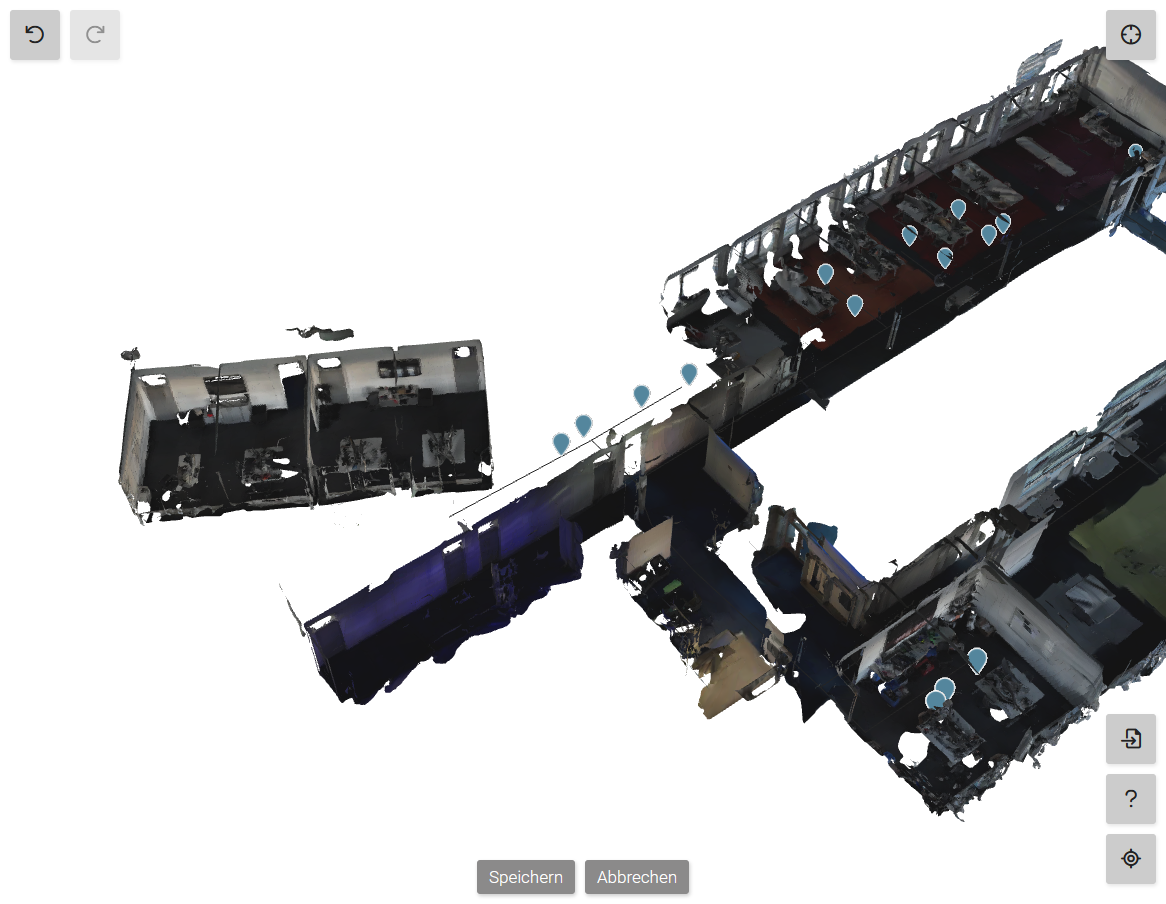
\includegraphics[width=0.9\textwidth]{Screenshot Editiermodus.png}
    \\
    Quelle: Eigene Darstellung
\end{figure}

Da der Boden bei allen 3D-Modellen ungefähr auf derselben z-Koordinate positioniert ist, müssen diese durch den Nutzer nicht weiter an der z-Achse verschoben werden. Im Vergleich zu den Roboterdaten sind die 3D-Modelle immer um 90° an der z-Achse und einen beliebigen Wert an der y-Achse rotiert, während die Rotation der x-Achse zwischen 3D-Modellen und Roboterdaten bereits übereinstimmt. Die 3D-Modelle werden im Editiermodus automatisch um -90° an der z-Achse rotiert und müssen vom Nutzer somit nur nach an der y-Achse rotiert werden. Die Roboterdaten und 3D-Modelle teilen sich bereits denselben Maßstab, weshalb der Nutzer nicht die Möglichkeit braucht die Modelle zu skalieren. Es gilt zu beachten, dass im Prototyp 3D-Modelle erwartet werden, die mit der Scaniverse App erzeugt wurden. In einem Produktivsystem sollten auch andere Quellen genutzt werden können. Die genannten Annahmen, dass die Modelle nicht um die z-Koordinate verschoben, nicht um die x- und z-Achse rotiert und nicht skaliert werden müssen, gelten dann nicht mehr. Somit bräuchte der Nutzer in einem Produktivsystem die Möglichkeit Modelle an allen Achsen zu verschieben und um alle Achsen zu rotieren. Auch müsste der Nutzer die Modelle skalieren können.

\subsection{Softwaretests}
Für eine größtmögliche Testabdeckung des entwickelten Prototyps wurden Unit und Integration Tests geschrieben. Das Testen der \deckgl{} Ansicht und Ebenen konnte nicht umgesetzt werden. So gibt es zwar den SnapshotTestRunner \cite{DeckglSnapshotTestRunner} mit dem das Framework testbar ist, dieser ist aber unzureichend dokumentiert, sodass die Tests nicht erfogreich implementiert werden konnten. Da die \deckgl{} Ansicht das Herzstück des Prototyps ist, ist die Testabdeckung unzureichend, aber unglücklicherweise auch nicht ausbaubar. Damit die Testabdeckung ausreicht muss erzwungenermaßen davon ausgegangen werden, dass die \deckgl{} Elemente ohne Fehler implementiert wurden. Es wurden Unit Tests für verschiedene Utility-Funktionen, für die komplexeren Redux Selektoren und für weitere Funktionen geschrieben. Die Redux Implementierung wurde bewusst nicht direkt getestet da es sich hierbei um Implementierungsdetails handelt die nach Kent C. Dodds nicht getestet werden sollten \cite{Dodds}. Stattdessen wird die Redux Implementierung zusammen mit den Buttons und dem Routenplanungs-Popup über Integration Tests getestet. Diese Vorgehensweise wird auch vom Redux Maintainer Mark Erikson empfohlen \cite{Erikson}. Die Unit und Integration Tests sind in die im Folgenden erklärte Deployment-Pipeline integriert.

\subsection{Deployment}
Für das Veröffentlichen des Prototyps wird GitHub Actions in Kombination mit GitHub Pages genutzt. Mit GitHub Actions lässt sich die Build-, Test- und Deployment-Pipeline eines Projekts automatisieren \cite{GitHubActions}. Bei GitHub Pages handelt es sich um einen Hosting-Dienst, der in GitHub integriert ist und aus Repositories statische Websites erstellen kann \cite{GitHubPages}. So wird mithilfe der actions-gh-pages Github Action \cite{ActionsGhPages} bei der Aktualisierung des Haupt-Branches automatisch ein Build erstellt. Das GitHub Repository ist so konfiguriert, dass der erstellte Build automatisch mit GitHub Pages veröffentlicht wird.

Die Anwendung verwendet verschiedene Funktionen der chayns-api \cite{ChaynsApi}, wie beispielsweise das Anfordern eines Zugangstokens, ohne den Funktionen des Backends nicht aufgerufen werden können. Diese Funktionen sind nur innerhalb der chayns Umgebung nutzbar, wesshalb die Anwendung nur funktioniert, wenn sie – wie in der Dokumentation des create-chayns-app Befehls beschrieben \cite{CreateChaynsApp} – als Custom Page auf einer chayns Seite eingebunden ist. Der Zugriff auf die meisten Endpunkte des \ac{BCB}s ist so eingeschränkt, dass diese nur von unternehmensinternen chayns Seiten aus aufgerufen werden können. Auf anderen chayns Seiten können die Steuerungs- und Verwaltungsfunktionen deshalb nicht oder nur eingeschränkt genutzt werden.
